% Figure 2 of the project summary: end-to-end flow.
\documentclass[border=2pt,10pt]{standalone}
\usepackage[T1]{fontenc}
\usepackage{newtxtext}
\usepackage{xcolor}
\usepackage{tikz}
\usetikzlibrary{arrows.meta,positioning,fit,backgrounds,calc,shapes.geometric}
\tikzset{
  box/.style={draw=black!75, rounded corners=2pt, align=center, font=\fontsize{9}{10.5}\selectfont, inner sep=3pt, fill=white},
  ext/.style={box, fill=black!4, dashed},
  arr/.style={-{Stealth[length=4pt]}, black!80, line width=0.55pt},
  lbl/.style={font=\fontsize{8.5}{9.5}\selectfont, inner sep=1.5pt},
  stage/.style={box, minimum height=0.88cm, text width=2.6cm},
  user/.style={stage, fill=green!6},
  m1/.style={stage, fill=blue!6},
  m2/.style={stage, fill=orange!8},
  dec/.style={box, diamond, aspect=2.0, fill=yellow!10, inner sep=1pt, text width=1.55cm},
}
\begin{document}
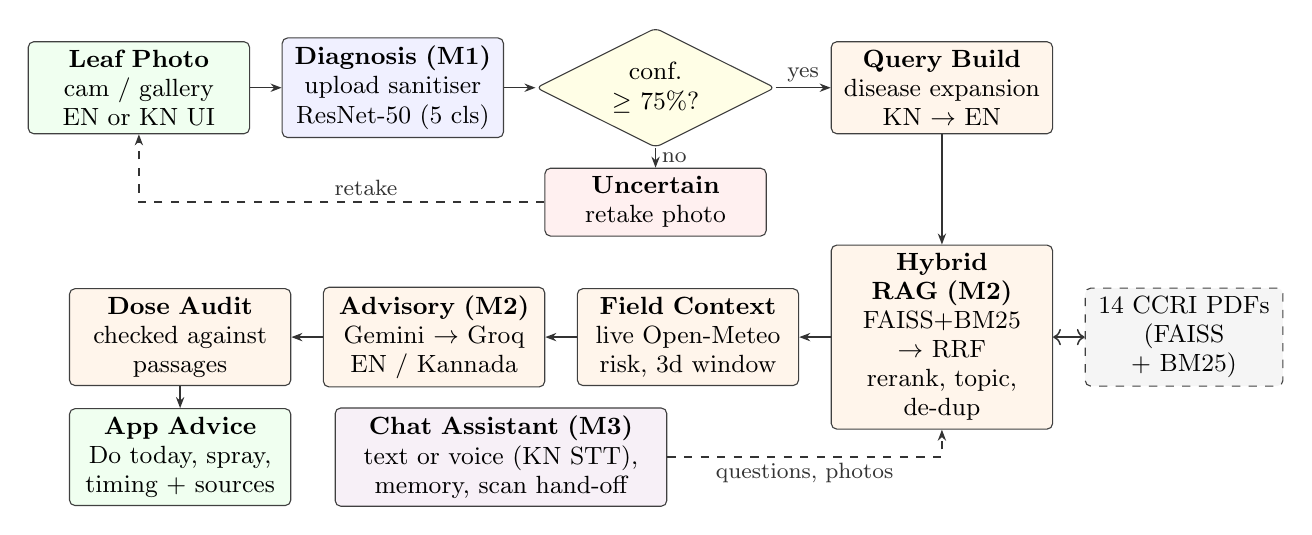
\begin{tikzpicture}
  % Row 1: photo -> diagnosis -> gate -> query
  \node[user] (photo) {\textbf{Leaf Photo}\\cam / gallery\\EN or KN UI};
  \node[m1, right=4mm of photo] (cnn) {\textbf{Diagnosis (M1)}\\upload sanitiser\\ResNet-50 (5 cls)};
  \node[dec, right=4mm of cnn] (gate) {conf.\\$\geq$ 75\%?};
  \node[m2, right=7mm of gate] (query) {\textbf{Query Build}\\disease expansion\\\mbox{KN $\rightarrow$ EN}};
  \node[box, fill=red!6, text width=2.6cm, below=2.5mm of gate] (unsure) {\textbf{Uncertain}\\retake photo};

  % Row 2: retrieval + weather -> LLM -> audit
  \node[m2, below=14mm of query] (ret) {\textbf{Hybrid RAG (M2)}\\FAISS+BM25 $\rightarrow$ RRF\\rerank, topic, de-dup};
  \node[ext, text width=2.3cm, minimum height=0.88cm, right=4mm of ret] (kb) {14 CCRI PDFs\\(FAISS + BM25)};
  \node[m2, left=4mm of ret] (wx) {\textbf{Field Context}\\live Open-Meteo\\risk, 3d window};
  \node[m2, left=4mm of wx] (llm) {\textbf{Advisory (M2)}\\Gemini $\rightarrow$ Groq\\EN / Kannada};
  \node[m2, left=4mm of llm] (audit) {\textbf{Dose Audit}\\checked against\\passages};

  % Row 3: output + chat assistant
  \node[user, below=2.8mm of audit] (out) {\textbf{App Advice}\\Do today, spray,\\timing + sources};
  \node[box, fill=violet!6, text width=4.0cm, minimum height=0.88cm, right=5.5mm of out] (chat)
       {\textbf{Chat Assistant (M3)}\\text or voice (KN STT),\\memory, scan hand-off};

  % Arrows
  \draw[arr] (photo) -- (cnn);
  \draw[arr] (cnn) -- (gate);
  \draw[arr] (gate) -- node[above=0.5pt, lbl]{yes} (query);
  \draw[arr] (gate) -- node[right=0.5pt, lbl]{no} (unsure);
  \draw[arr] (query) -- (ret);
  \draw[arr, <->] (ret) -- (kb);
  \draw[arr] (ret) -- (wx);
  \draw[arr] (wx) -- (llm);
  \draw[arr] (llm) -- (audit);
  \draw[arr] (audit) -- (out);
  \draw[arr, dashed] (chat.east) -| node[pos=0.25, below=0.5pt, lbl]{questions, photos} (ret.south);
  \draw[arr, dashed] (unsure.west) -| node[pos=0.22, above=0.5pt, lbl]{retake} (photo.south);
\end{tikzpicture}
\end{document}
